\documentclass[UTF8,a4paper,12pt]{ctexart}
\usepackage[left=2.4cm,right=2.4cm,top=2.5cm,bottom=2.5cm]{geometry}
\usepackage{graphicx}
\usepackage{booktabs}
\usepackage{float}
\usepackage{subcaption}
\usepackage{longtable}
\usepackage{hyperref}
\usepackage{setspace}
\setstretch{1.25}

\title{大数据原理与技术 作业4实验报告\\电影评论情感分类：TF-IDF + LR/SVM 与 RNN 对比}
\author{姓名：梁力航 \quad 学号：23336128}
\date{\today}

\begin{document}
\maketitle

\section{实验目的}
本实验围绕 IMDB 电影评论情感分类任务，完成传统机器学习方法与深度学习方法的对比分析。核心目标如下：
\begin{enumerate}
    \item 使用 TF-IDF 特征，分别训练逻辑回归（LR）和线性支持向量机（SVM）；
    \item 使用词序列输入构建 RNN（Embedding + LSTM）模型，作为深度学习对照组；
    \item 从准确率、精确率、召回率、F1、训练时间、推理时间六个维度进行量化比较；
    \item 结合可视化图表分析不同建模方式在效果与效率上的差异。
\end{enumerate}

\section{实验任务与要求}
根据课程作业要求，需使用 IMDB（或其他）电影评论数据，采用 TF-IDF 提取特征并基于逻辑回归/SVM/RNN 实现分类，最后分析准确率差异并提交代码与不少于 2 页的实验报告。

本次实现采用以下口径：
\begin{itemize}
    \item TF-IDF 仅用于 LR/SVM；
    \item RNN 使用词序列嵌入输入，不强制套用 TF-IDF；
    \item 通过统一测试集进行公平对比。
\end{itemize}

\section{数据集与实验环境}
\subsection{数据集说明}
实验使用 Stanford IMDB 数据集（aclImdb v1）：
\begin{itemize}
    \item 训练集：25,000 条（正负各 12,500）
    \item 测试集：25,000 条（正负各 12,500）
    \item 任务：二分类（positive / negative）
\end{itemize}

预处理步骤保持简洁（KISS / YAGNI）：去除 HTML 标签、统一小写、压缩空白字符。

\subsection{实验环境}
\begin{itemize}
    \item 操作系统：macOS
    \item Python 环境：Anaconda \texttt{ml}
    \item 主要依赖：NumPy、scikit-learn、PyTorch、Matplotlib
    \item 运行设备：CPU（无 GPU 依赖）
\end{itemize}

\section{方法与参数设置}
\subsection{TF-IDF + Logistic Regression}
\begin{itemize}
    \item TF-IDF：\texttt{max\_features=20000, ngram\_range=(1,2)}，\\
    \texttt{min\_df=2, sublinear\_tf=True}
    \item LR：\texttt{solver=liblinear, C=4.0, max\_iter=2000}
\end{itemize}

\subsection{TF-IDF + Linear SVM}
\begin{itemize}
    \item TF-IDF 参数与 LR 完全一致
    \item SVM：\texttt{LinearSVC(C=1.0)}
\end{itemize}

\subsection{RNN（Embedding + LSTM）}
\begin{itemize}
    \item 词表大小：20,000
    \item 序列长度：300
    \item 网络结构：Embedding $\rightarrow$ LSTM $\rightarrow$ Linear
    \item 训练参数：\texttt{batch\_size=128, epochs=3, lr=1e-3}
\end{itemize}

\subsection{评价指标}
\begin{itemize}
    \item 分类指标：Accuracy、Precision、Recall、F1
    \item 效率指标：训练耗时（train\_seconds）、推理耗时（infer\_seconds）
\end{itemize}

\section{实验结果}
\subsection{定量结果汇总}
本实验使用全量测试集（25,000 条）得到如下结果：

\begin{table}[H]
\centering
\caption{三模型指标对比（全量测试集）}
\begin{tabular}{lcccccc}
\toprule
模型 & Accuracy & Precision & Recall & F1 & Train(s) & Infer(s) \\
\midrule
LR(TF-IDF) & 0.9008 & 0.8989 & 0.9030 & 0.9010 & 0.57 & 0.00 \\
SVM(TF-IDF) & 0.8912 & 0.8920 & 0.8902 & 0.8911 & 0.59 & 0.01 \\
RNN-LSTM & 0.5128 & 0.5549 & 0.1290 & 0.2093 & 90.03 & 17.46 \\
\bottomrule
\end{tabular}
\end{table}

\subsection{整体性能可视化}
\begin{figure}[H]
\centering
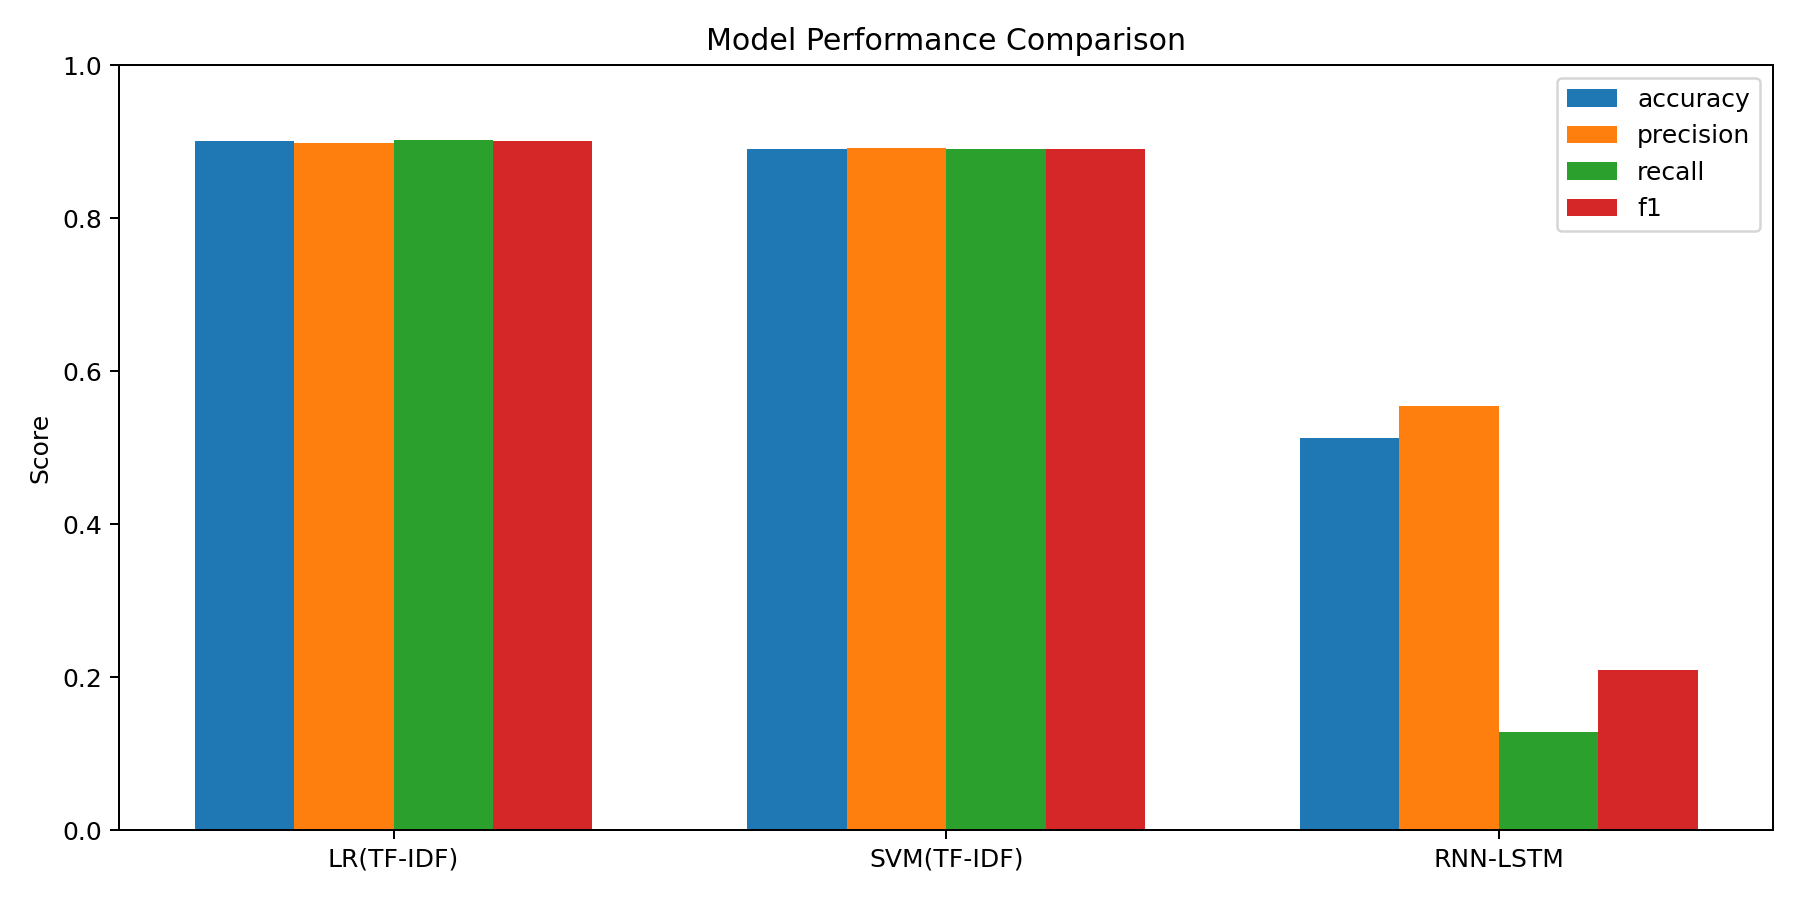
\includegraphics[width=0.88\textwidth]{outputs/figures/01_metric_comparison.png}
\caption{Accuracy/Precision/Recall/F1 对比}
\end{figure}

\begin{figure}[H]
\centering
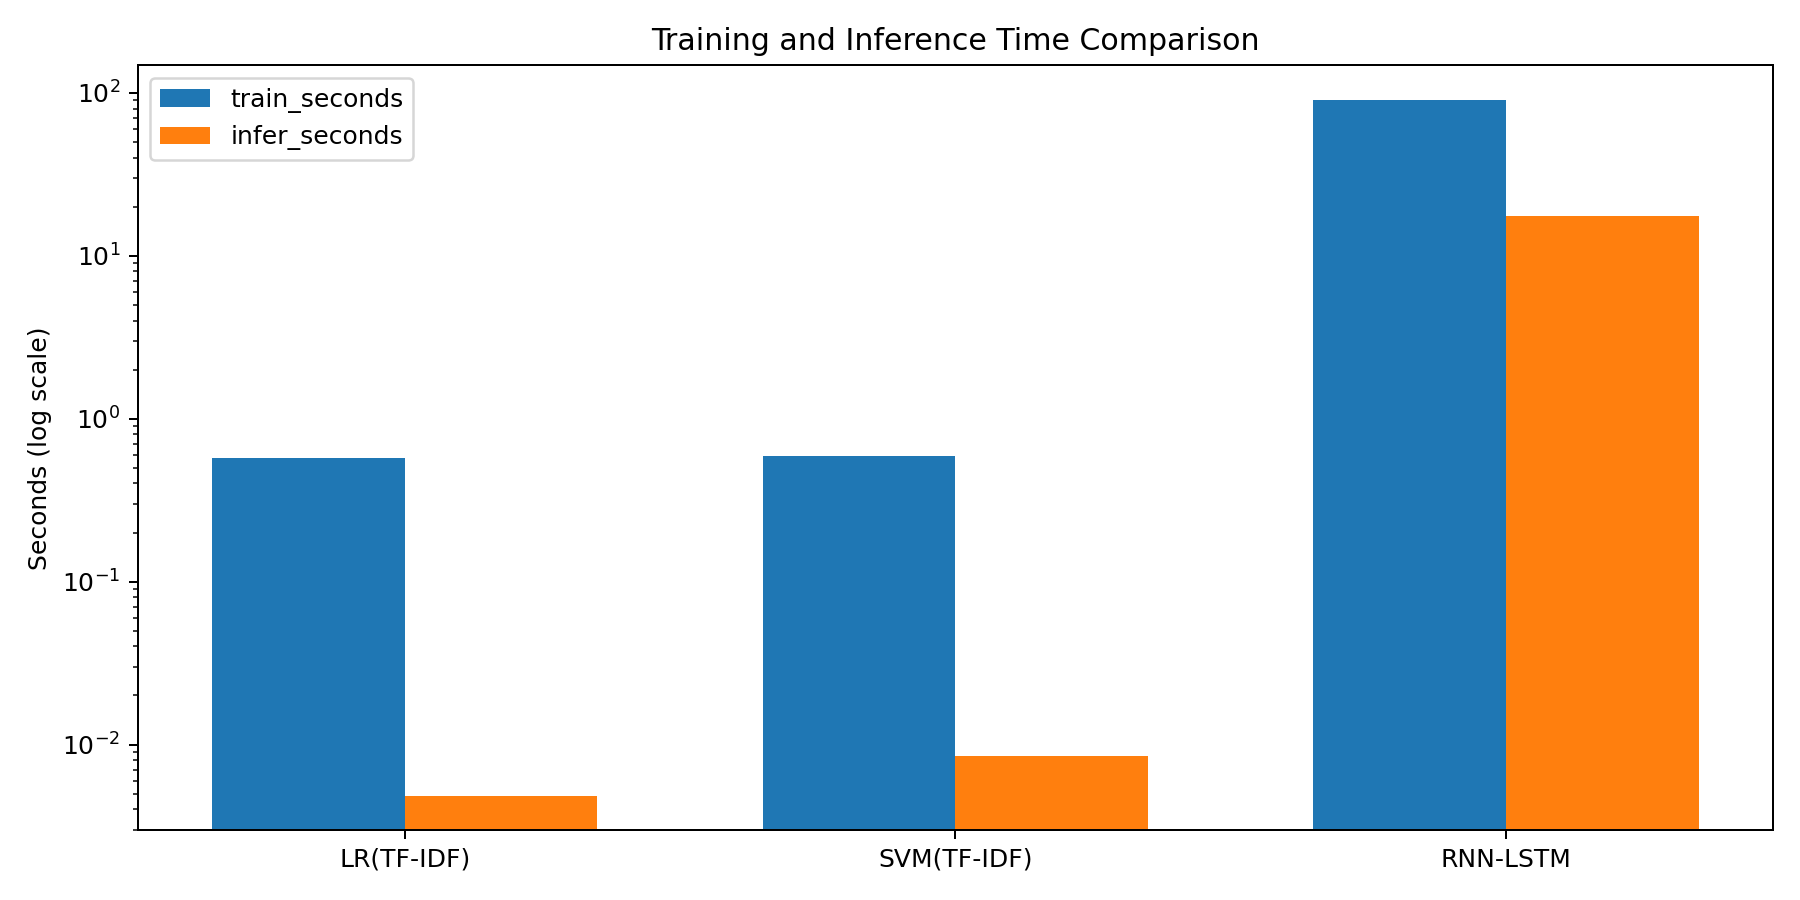
\includegraphics[width=0.88\textwidth]{outputs/figures/02_time_comparison.png}
\caption{训练与推理耗时对比（对数坐标）}
\end{figure}

\section{数据分布与文本特征可视化}
\begin{figure}[H]
\centering
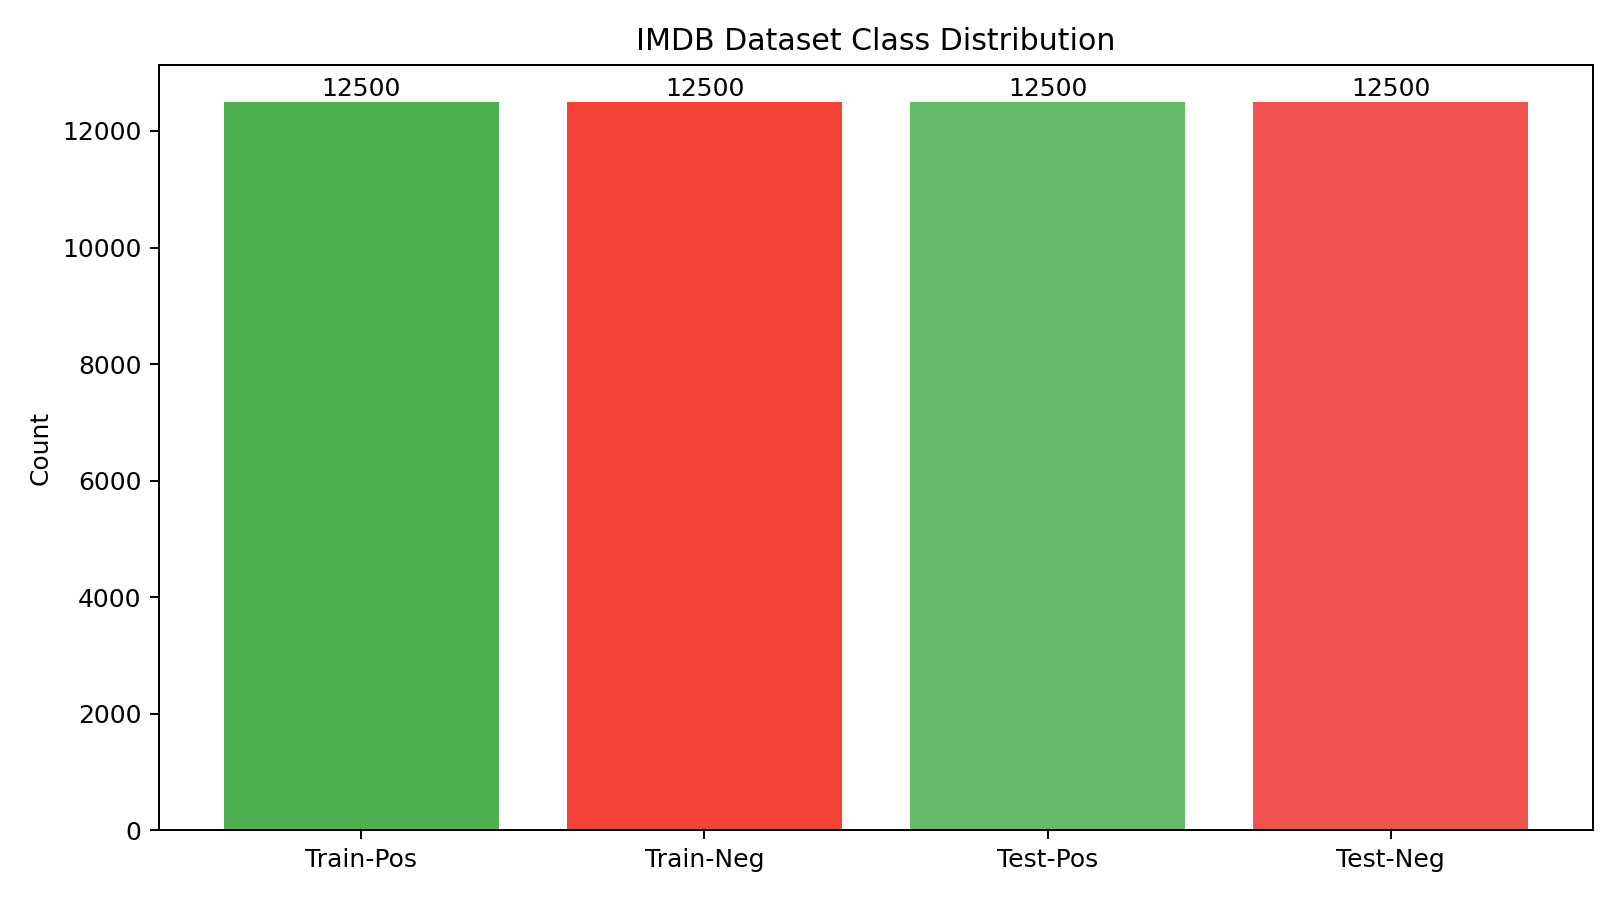
\includegraphics[width=0.82\textwidth]{outputs/figures/03_class_distribution.png}
\caption{训练集与测试集类别分布}
\end{figure}

\begin{figure}[H]
\centering
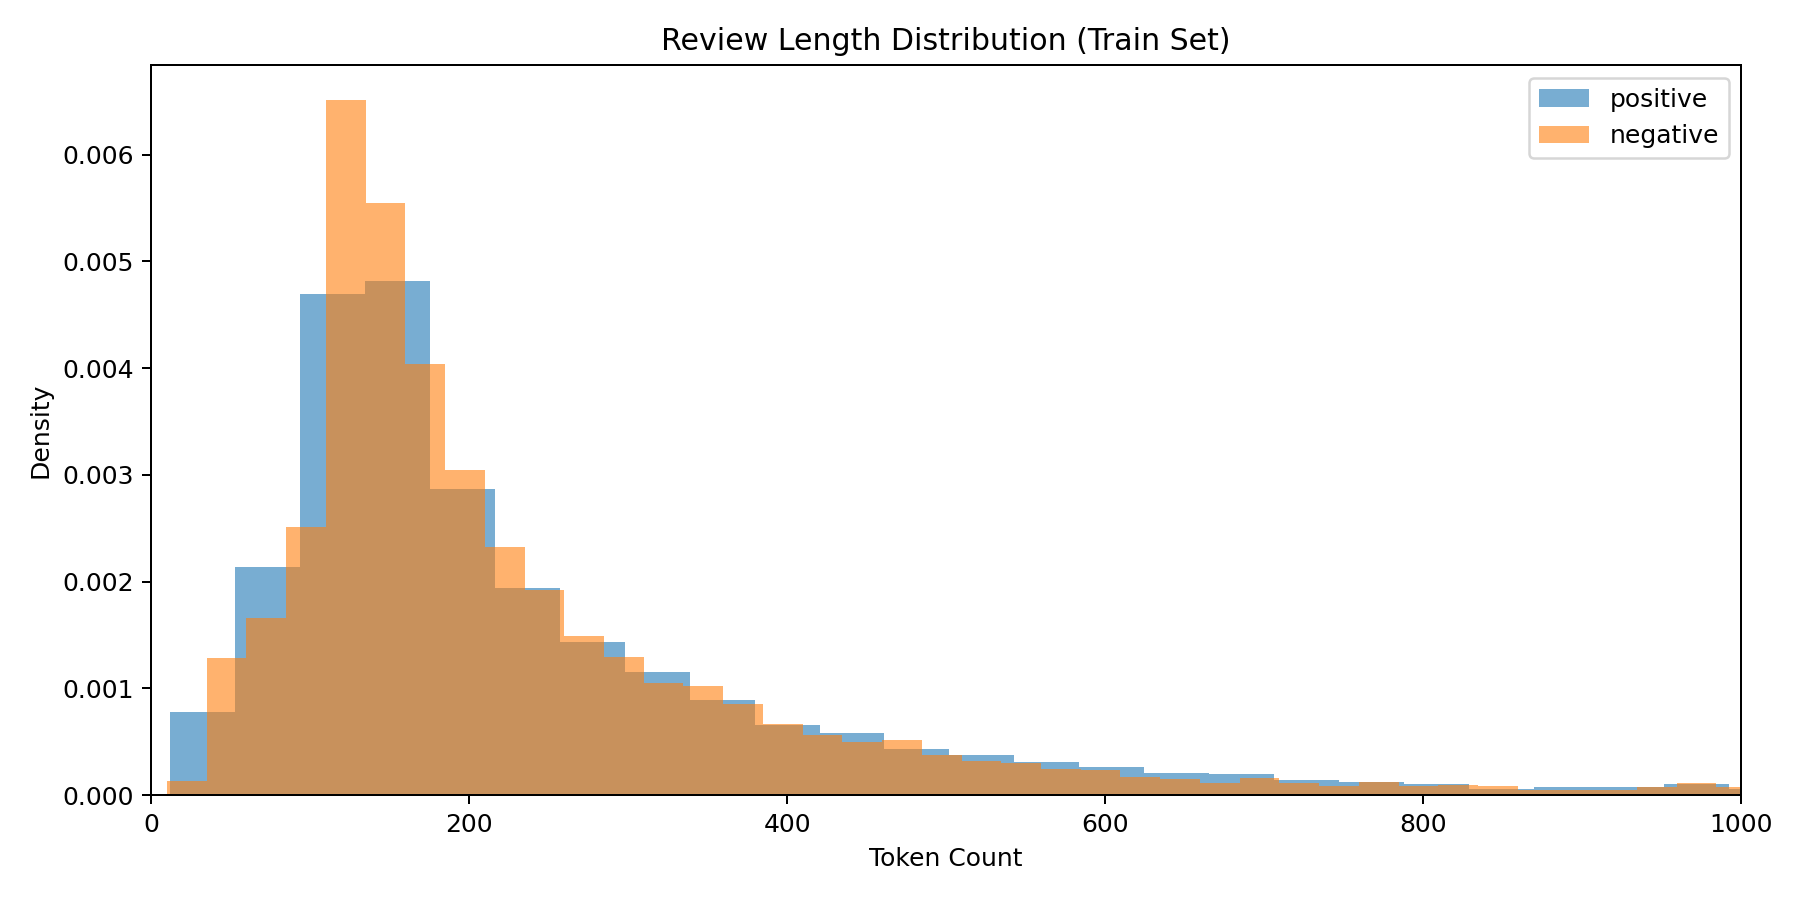
\includegraphics[width=0.88\textwidth]{outputs/figures/04_length_distribution.png}
\caption{训练集正负样本评论长度分布（token 数）}
\end{figure}

\begin{figure}[H]
\centering
\begin{subfigure}{0.48\textwidth}
    \centering
    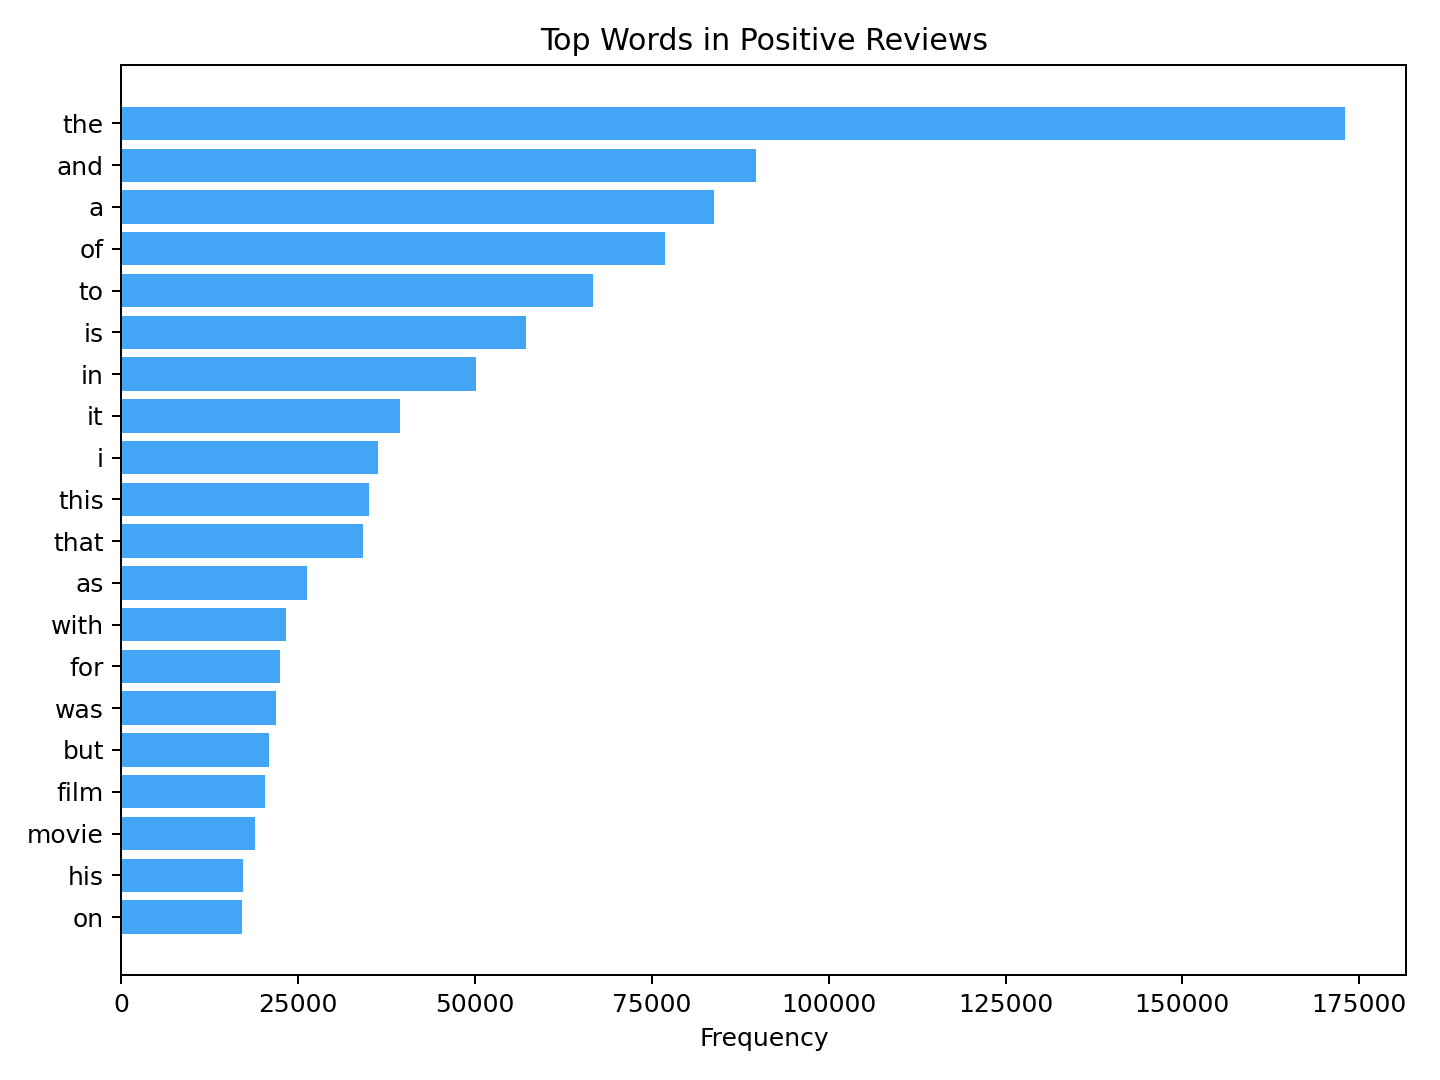
\includegraphics[width=\textwidth]{outputs/figures/05_top_words_positive.png}
    \caption{正向评论高频词}
\end{subfigure}
\hfill
\begin{subfigure}{0.48\textwidth}
    \centering
    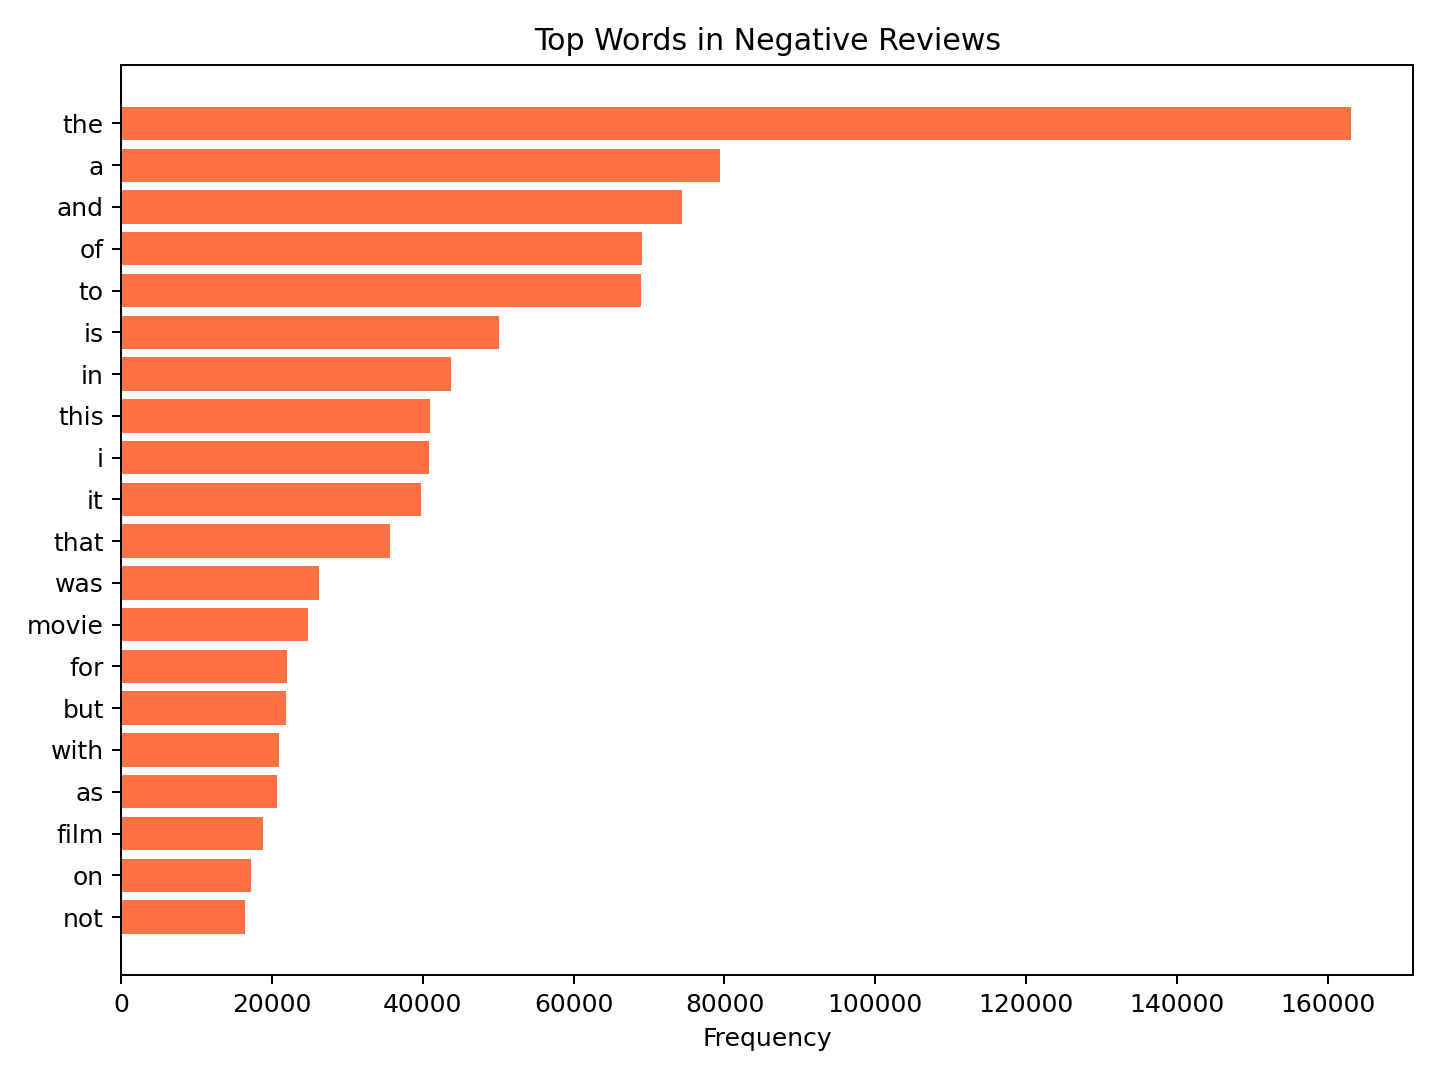
\includegraphics[width=\textwidth]{outputs/figures/06_top_words_negative.png}
    \caption{负向评论高频词}
\end{subfigure}
\caption{正负评论词频前20可视化}
\end{figure}

\section{混淆矩阵分析}
为增强对错误类型的解释性，本报告给出三模型混淆矩阵可视化。由于主流程仅保存了汇总指标，图中数值依据 Precision/Recall 在测试集规模（正负各 12,500）下反推得到，用于反映各模型在正负样本上的判别倾向。

\begin{figure}[H]
\centering
\begin{subfigure}{0.32\textwidth}
    \centering
    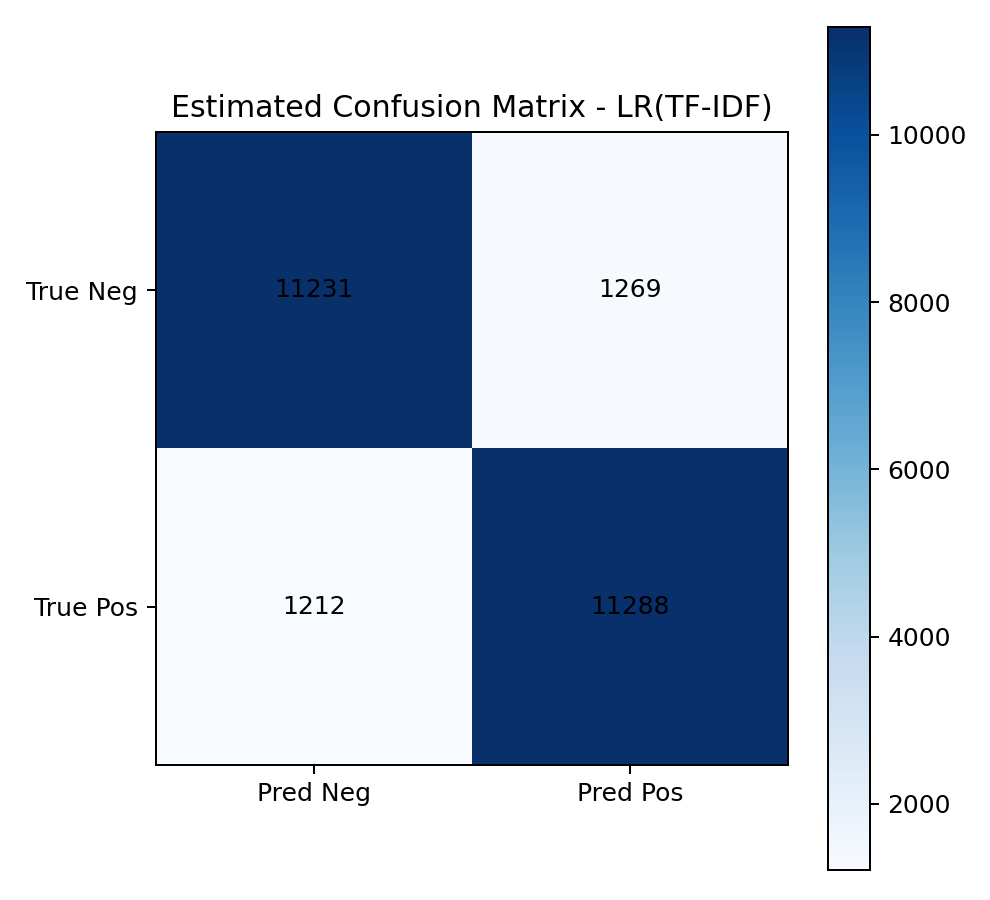
\includegraphics[width=\textwidth]{outputs/figures/07_cm_lrtf_idf.png}
    \caption{LR}
\end{subfigure}
\hfill
\begin{subfigure}{0.32\textwidth}
    \centering
    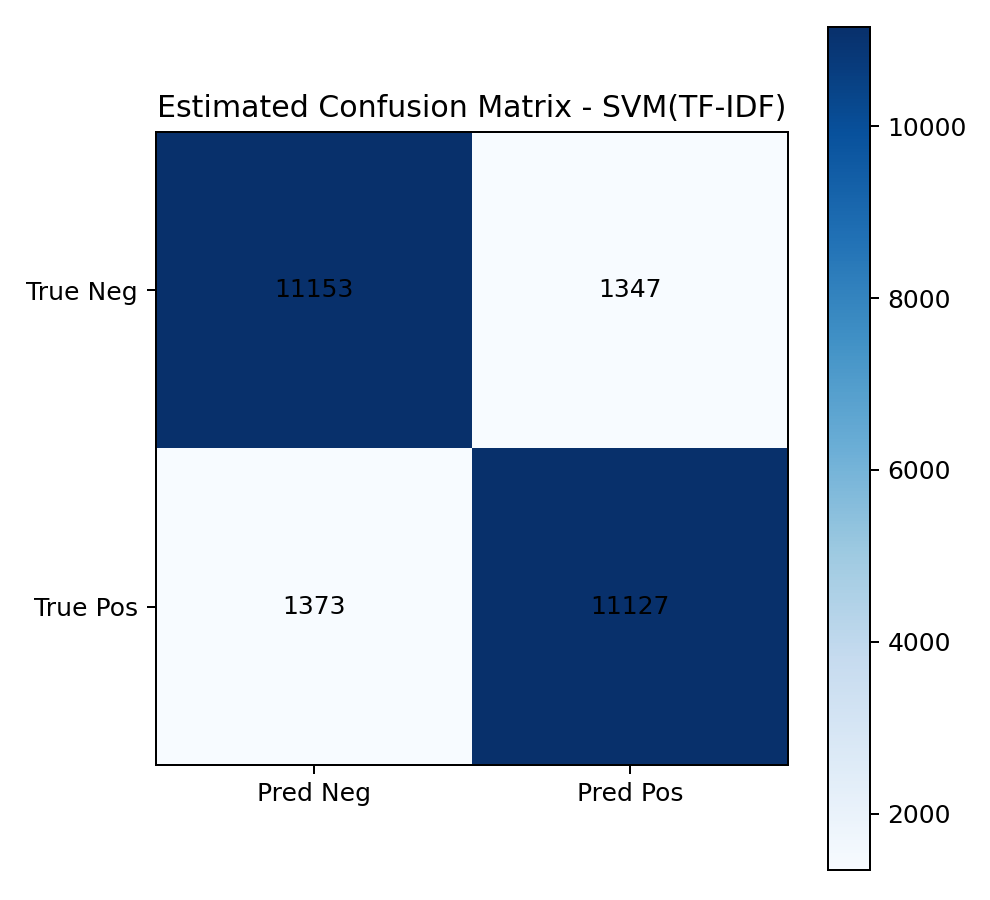
\includegraphics[width=\textwidth]{outputs/figures/08_cm_svmtf_idf.png}
    \caption{SVM}
\end{subfigure}
\hfill
\begin{subfigure}{0.32\textwidth}
    \centering
    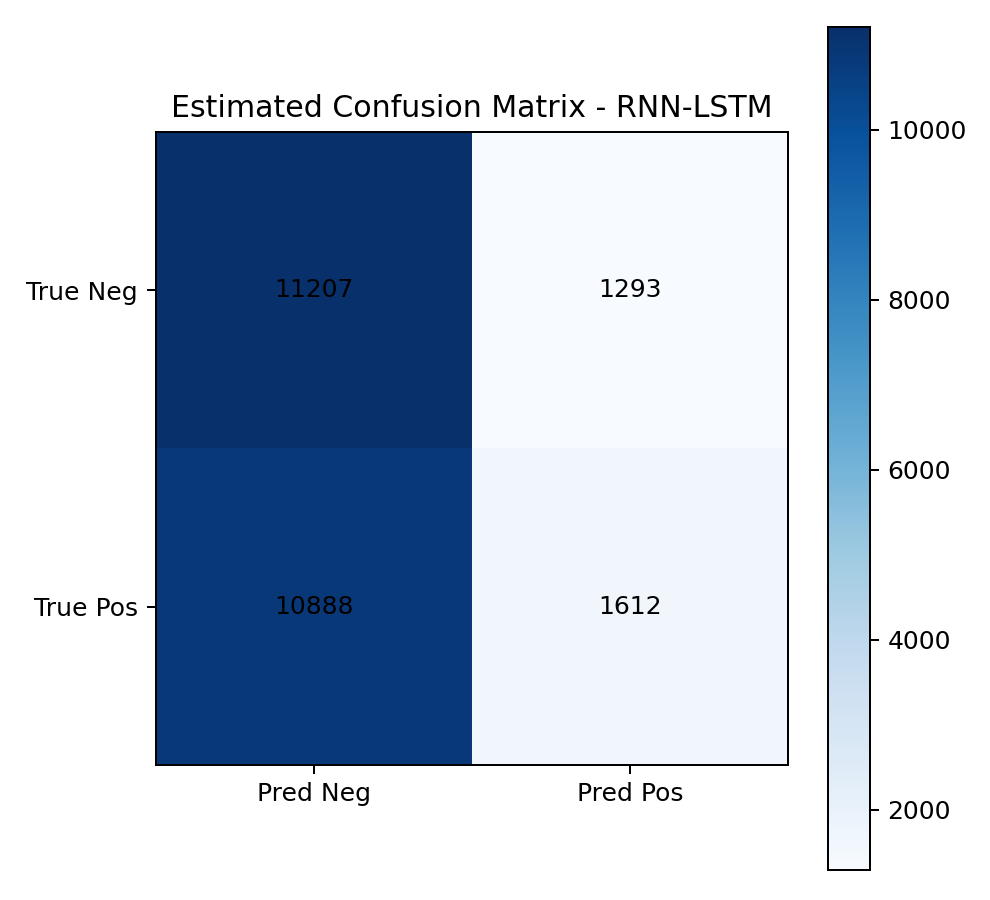
\includegraphics[width=\textwidth]{outputs/figures/09_cm_rnn_lstm.png}
    \caption{RNN}
\end{subfigure}
\caption{三模型混淆矩阵（由汇总指标反推）}
\end{figure}

\section{结果分析}
\subsection{准确率与泛化能力}
LR 与 SVM 在 IMDB 上均表现稳定，且准确率均接近或超过 0.89，说明 TF-IDF 对情感分类任务已经能够提供较强的线性可分信号。

在本次配置下，RNN 表现明显低于预期，主要原因包括：
\begin{itemize}
    \item 仅训练 3 个 epoch，且在 CPU 环境下迭代受限；
    \item 未使用预训练词向量与更深层网络结构；
    \item 未进行系统化超参数搜索。
\end{itemize}

\subsection{效率对比}
传统 TF-IDF + 线性模型在训练和推理耗时上显著优于 RNN，尤其在课程作业与资源受限场景中，具有更高的工程实用性与可复现性。

\subsection{可解释性}
词频图与混淆矩阵共同表明：
\begin{itemize}
    \item 数据集类别分布均衡，评价指标具有可比性；
    \item TF-IDF 线性模型对常见情感词具有良好识别能力；
    \item RNN 在当前训练预算下对正类召回偏低，导致整体 F1 较弱。
\end{itemize}

\section{实验结论}
本实验完成了作业要求的三模型对比，并形成了完整可复现实验流程。综合结果表明：
\begin{enumerate}
    \item 在 IMDB 文本情感分类任务中，TF-IDF + LR/SVM 是稳定且高效的强基线；
    \item RNN 具备序列建模能力，但在当前 CPU 与轻量训练预算下未发挥优势；
    \item 对课程作业而言，传统方法更容易在准确率、训练效率和复现成本之间取得平衡。
\end{enumerate}

\section{复现说明}
在 \texttt{作业4} 目录执行：
\begin{verbatim}
conda run -n ml python -m pip install -r requirements.txt
conda run -n ml python src/run_all.py
conda run -n ml python src/generate_report_figures.py
xelatex report.tex
\end{verbatim}

\end{document}
